%- block legend
Douglas está muito preocupado com um grande vazamento de senhas de sua rede
social favorita. Por isso, ele
decidiu que irá escolher uma nova senha para sua rede.
Metódico que é, Douglas decidiu que irá escolher sua nova senha usando seu
\textit{disco de senha}, que é um disco circular contendo $N$ letras minúsculas.
A senha será escolhida da seguinte forma:
\begin{enumerate}
    \item Douglas irá escolher alguma letra no disco para ser a primeira letra
    da senha;
    \item A senha será formada percorrendo o disco em sentido horário, a partir
    da primeira letra, concatenando as letras percorridas;
    \item A senha deverá ter no mínimo 1 e no máximo $K$ letras.
\end{enumerate}

Quantas senhas \textit{distintas} podem ser formadas dessa maneira?

%- endblock

%- block input
A primeira linha contém dois inteiros $N$ e $K$ ($1 \leq K \leq N \leq
        \VAR{vars.N.max | sci}$), o número de letras no disco e o tamanho máximo
da senha, respectivamente.
A segunda linha contém $N$ letras minúsculas indicando as letras no disco, em
sentido horário, a partir de qualquer uma delas.
%- endblock

%- block output
Imprima uma linha com o número de senhas distintas que podem ser formadas.
%- endblock

%- block notes
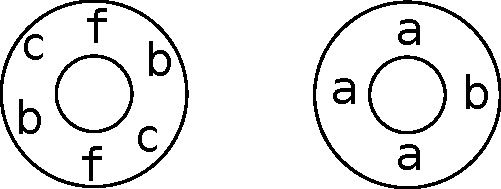
\includegraphics[scale=0.6]{disco0.pdf}\\
Os discos acima representam os dois primeiros exemplos de entrada.
No primeiro exemplo, as senhas que podem ser formadas com até $K=3$ letras são
\texttt{b}, \texttt{c}, \texttt{f}, \texttt{bc}, \texttt{cf}, \texttt{fb},
\texttt{bcf}, \texttt{cfb} e \texttt{fbc}, totalizando 9 senhas distintas.
No segundo exemplo, as senhas que podem ser formadas com até $K=2$ letras são
\texttt{a}, \texttt{b}, \texttt{aa}, \texttt{ab} e \texttt{ba}, totalizando 5 senhas distintas.

%- endblock

%- block editorial
Primeiramente, vamos remover a condição de que a string é circular concatenando
a string com ela mesma. No primeiro exemplo de entrada, vamos transformar a
string $S=$\texttt{fbcfbc} em $S=$\texttt{fbcfbcfbcfbc}. O problema se reduz agora a
contar quantas substrings distintas de tamanho máximo $K$ existem em $S$.

O \textit{vetor de sufixos} (\textit{Suffix Array}) de uma string $S$ é o vetor
de todos os sufixos de $S$, em ordem lexicografica crescente. Como exemplo, o
vetor de sufixos de \texttt{fbcfbcfbcfbc} é:

\begin{verbatim}
 0:
 1: bc
 2: bcfbc
 3: bcfbcfbc
 4: bcfbcfbcfbc
 5: c
 6: cfbc
 7: cfbcfbc
 8: cfbcfbcfbc
 9: fbc
10: fbcfbc
11: fbcfbcfbc
12: fbcfbcfbcfbc
\end{verbatim}

Não é necessário armazenar cópias da string em cada posição do vetor, mas sim
apenas em qual posição em $S$ o sufixo começa.

Note que toda substring de $S$ é prefixo de algum de seu sufixo! Por exemplo, no
sufixo \texttt{bcfbc} estão as substrings \texttt{b}, \texttt{bc}, \texttt{bcf},
\texttt{bcfb} e \texttt{bcfbc}.

Vamos construir a resposta de maneira incremental, percorrendo o vetor de
sufixos em ordem; para cada sufixo processado, vamos incrementar na resposta a
quantidade de \textbf{novas} substrings de tamanho máximo $K$ contidas no
sufixo (as que ainda não foram ``vistas'' anteriormente).

Para cada sufixo na posição $i$ do vetor de sufixos, seja $LCP_i$ o tamanho do maior prefixo comum (\textit{Longest Commom
Prefix}) de $i$ com o sufixo $i-1$ no vetor de sufixos. Como exemplo,
$LCP_2 = 2$ no exemplo dado, uma vez que o maior prefixo comum do sufixo na
posição $2$ (\texttt{bcfbc}) com o da posição $1$ (\texttt{bc}) tem tamanho 2;
Como exemplo exemplo, $LCP_6 = 1$; etc.

Para cada sufixo na posição $i$, note que todas as substrings nesse sufixo que
tem tamanho até $LCP_i$ já foram ``vistas'' em iterações anteriores; assim, há
$min\{K,|$sufixo$|\} - LCP_i$ \textbf{novas} substrings de tamanho máximo $K$ no
sufixo $i$ (ou nenhuma se $LCP_i \geq k$).

Uma referência para o algoritmo de construção do vetor de sufixos e cálculo de
$LCP$ é:

\url{https://www.geeksforgeeks.org/competitive-programming/suffix-arrays-for-competitive-programming/}

O problema pode ser resolvido em $O(N\lg N)$, mas a solução $O(N\lg^2 N)$ é
rápida o bastante para os limites deste problema.
%- endblock
